\documentclass[handout]{beamer}
\usepackage{verbatim}
\usepackage{xcolor}
\usepackage{multirow}
\usepackage{amssymb}
\usepackage{tikz}
\usetikzlibrary{positioning,fit}
%\usepackage{enumitem}
\usetheme{Warsaw}
\setbeamertemplate{navigation symbols}{}
\newcommand{\blue}[1]{{\color{blue} #1}}
\newcommand{\red}[1]{{\color{red} #1}}
\newcommand{\grn}[1]{{\color{green} #1}}
\newcommand{\bluRed}[2]{{\color{blue} #1}{\color{red} #2}}
\newcommand{\qtns}[0]{\begin{center} Questions? \end{center}}
\newcommand{\nl}[1]{\vspace{#1 em}}
\newcommand{\cntrImg}[2]{\begin{center}\includegraphics[scale=#2]{#1}\end{center}}
\newcommand{\defn}[1]{{\bf #1}}
\let\emptyset\varnothing
\newcommand{\SampS}[0]{$\mathcal{S}$}

\title{Math 3070, Applied Statistics}

\begin{document}

\begin{frame}
    \begin{beamercolorbox}[rounded=true,wd=\textwidth,center]{title}
        \usebeamerfont{title}\inserttitle
    \end{beamercolorbox}
    \begin{center}
        Section 1\\
        \nl{0.5}
        August 28, 2019
    \end{center}

\end{frame}

\begin{frame}{Lecture Outline, 8/28}
    Section 2.4
    \begin{itemize}
        \item Conditional Probability and Multiplication Rule
        \item Law of Total Probability and Bayes' Theorem
        \item Questions about Quiz Materials
    \end{itemize}
\end{frame}

\begin{frame}{Conditional Probability}
    Goal: Compute probabilities of events when another event has occured.
    \\
    \nl{0.5}
    Notation: $P(A|B)$ represents the conditional probability of event $A$ given that the event $B$ has occured.
    \\
    \nl{0.5}
    \pause Example: 
    \[A = \text{"six-sided die lands on 2"} = \{2\}\] 
    \[B = \text{"six-sided die lands on an even number"} = \{2,4,6\}\]
    \[P(B|A) = \pause 1\]
    \[P(A|B) = \pause \frac{1}{3}\]
    There are three even numbers so we expect that the probability that two is one of them is $\frac{1}{3}$ when an even number must land.
\end{frame}

\begin{frame}{Conditional Probability, Definition}
    \begin{center}
\begin{tabular}{ c c}
    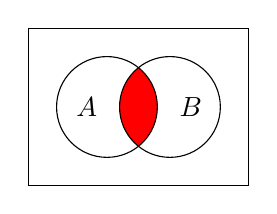
\begin{tikzpicture}[scale=.4]
        \def\firstcircle{(180:1cm) circle (1.6cm)}
          \def\secondcircle{(0:1cm) circle (1.6cm)}
             \begin{scope}
                \clip \firstcircle;
                \fill[red] \secondcircle;
            \end{scope}
              \draw \firstcircle node[text=black,left] {$A$};
              \draw \secondcircle node [text=black,right] {$B$};
              \draw (-3.5,-2.5) rectangle (3.5,2.5);
        \end{tikzpicture}
&
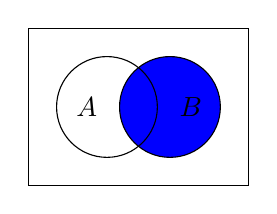
\begin{tikzpicture}[scale=.4]
    \def\firstcircle{(180:1cm) circle (1.6cm)}
      \def\secondcircle{(0:1cm) circle (1.6cm)}
    \def\mainrect{(-3.5,-2.5) rectangle (3.5,2.5)}
          \fill[blue] \secondcircle;
          \draw \firstcircle node[text=black,left] {$A$};
          \draw \secondcircle node [text=black,right] {$B$};
          \draw (-3.5,-2.5) rectangle (3.5,2.5);
    \end{tikzpicture}
    \\
\end{tabular}
\end{center}
\begin{definition}
    Let $B$ be an event with $P(B)>0$. The \textbf{conditional probability} that an event $A$ occurs, given that $B$ occurs, is
    $$P(A|B)=\frac{\red{P(A\cap B)}}{\blue{P(B)}}$$
    Multiplication Rule: $P(A\cap B) = P(A|B)\cdot P(B)$
\end{definition}
\end{frame}

\begin{frame}{Conditional Probability, Intuition}
    Intuition: event $B$ has occured the only outcomes in event $A$ that can occur must also be in event $B$, $A\cap B$. Since event $B$ has occured, the number of possible outcomes is the number of outcomes in $B$.

    \pause \[P(A|B) = \frac{\text{\# of outcomes in } A\cap B}{\text{\# of outcomes in } \mathcal{S}} \bigg/ \frac{\text{\# of outcomes in } B}{\text{\# of outcomes in } \mathcal{S}}\]
    \[ = \frac{\text{\# of outcomes in } A\cap B}{\text{\# of outcomes in } B}\]
\end{frame}

\begin{frame}{Conditional Probability, Verification Example}
Example: Use the formula to verify the previous example.
    \[A = \text{"six-sided die lands on 2"} = \{2\}\] 
    \[B = \text{"six-sided die lands on an even number"} = \{2,4,6\}\]
    \[P(A) = \frac{1}{6} \hskip 1em P(B) = \frac{3}{6} \hskip 1em P(A \cap B) = \frac{1}{6}\]
    \pause \[P(A|B) = \frac{P(A\cap B)}{B} = \frac{1/6}{3/6} = \frac{1}{3}\]
    \[P(B|A) = \frac{P(A\cap B)}{A} = \frac{1/6}{1/6} = 1\]
\end{frame}

\begin{frame}{Conditional Probability, Multiplication Rule Example}
    Problem: The 2010 US Census found that 23\% of US residents are undergraduate students. CNBC reports that 73\% of undergraduate students have student loans. Determine the probability that a randomly selected person is an undergraduate student and has student loans. \\
    \nl{0.5}
    \begin{center}
        event $A =$ "some one with student loans is selected"\\ \nl{0.5}
        event $B =$ "an undergraduate student is selected"
    \end{center}
    \[P(A \cap B) = P(A|B) \cdot P(B) = \pause 0.73 \cdot 0.23 = 0.1679\]
    \end{frame}

    \begin{frame}{Conditional Probability, Multiplication Rule Example}
        Problem: The 2010 US Census found that 23\% of US residents are undergraduate students. CNBC reports that 73\% \blue{of undergraduate students} \red{have student loans}. Determine the probability that a randomly selected person is an undergraduate student and has student loans. \\
        \nl{0.5}
        \begin{center}
            event $A =$ "some one with student loans is selected"\\ \nl{0.5}
            event $B =$ "an undergraduate student is selected"
        \end{center}
        \[P(A \cap B) = P(\red{A}|\blue{B}) \cdot P(B) = \pause 0.73 \cdot 0.23 = 0.1679\]
    \end{frame}

    \begin{frame}{Conditional Probability, Summary}
        \begin{itemize} 
            \item Conditional Probability and Multiplication Formula, respectively,
            \[P(A|B) = \frac{P(A\cap B)}{P(B)} \text{ and } P(A \cap B) = P(A|B) P(B)\]
            \item Used when a condition is given, must happen or always true.
            \item Homework Hint: event $A$ from the verification example is contained inside event $B$.
        \end{itemize}
        \qtns
    \end{frame}

    \begin{frame}{Law of Total Probability, Explanation}
        \begin{block}{}
        Let $A_1,\dots,A_n$ be disjoint events with $\mathcal{S}=A_1\cup\cdots\cup A_n$ ($A_i$ \textbf{partition} $\mathcal {S}$). Then for any event $B$,
        $$P(B)=\sum_{i=1}^n P(A_i)P(B|A_i)$$
        picture on page 80
        \end{block}
        
        Proof: By the multiplication rule, \begin{align*}
        \sum_{i=1}^n P(A_i)P(B|A_i) &= 
        \sum_{i=1}^n P(A_i) \frac{P(A_i \cap B)}{P(A_i)} \\
        &= P(A_1\cap B)+\cdots+P(A_n\cap B)\\
        (B\cap A_i\text{ are disjoint})&= P((A_1\cap B)\cup\cdots\cup (A_n\cap B)) \\
        &= P((A_1 \cup \cdots \cup A_n) \cap B) \\
        &= P(\mathcal{S} \cap B) = P(B)
        \end{align*}
    \end{frame}

    \begin{frame}{Law of Total Probability, Complement Example}
        Problem: The probability of \red{seeing the sun is 9\% when there is rain} and \grn{65\% when there is no rain}. The probability that there is \blue{rain today is 60\%}. What is the probability of seeing the sun?
        \pause \begin{center}
            event $A =$ "seeing the sun"\\ \nl{0.5}
            event $B =$ "there is rain today"
        \end{center}
        \begin{enumerate}
            \pause \item $B$ and $B'$ partition $\mathcal{S}$
            \pause \item $P(B') = 1 - P(B) = 1 - 0.6 = 0.4$
            \pause \item \begin{align*}
                P(A) &= P(B)P(A|B)+P(B')P(A|B') \\
                 &= \blue{0.6}\cdot \red{0.09}+0.4\cdot \grn{0.65}\\
                 & = 0.314\\
            \end{align*}
        \end{enumerate}
    \end{frame}

    \begin{frame}{Law of Total Probability, Example}
        Problem: Select flipping 1,2 or 3 fair coins, equally likely. What is the probability that at all coins land on heads?
        \pause \begin{center}
            event $A_i =$ i "coins selected"\\ \nl{0.5}
            event $B =$ "all coins land on heads"
        \end{center}
        \begin{enumerate}
            \pause \item $P(A_i) = \pause \frac{1}{3}$
            \pause \item $P(B|A_1) = \pause \frac{1}{2}$
            \pause \item $P(B|A_2) = \pause \frac{1}{4}$
            \pause \item $P(B|A_2) = \pause \frac{1}{8}$
            \pause \item \begin{align*}
                P(B) &= P(A_1)P(B|A_1)+P(A_2)P(B|A_2)+P(A_3)P(B|A_3) \\
                 \pause &= \frac{1}{3}\frac{1}{2} + \frac{1}{3}\frac{1}{4} + \frac{1}{3}\frac{1}{8} = \frac{1}{3}\bigg(\frac{1}{2} + \frac{1}{4} + \frac{1}{8}\bigg)\\
                 & \approx 0.291666667
            \end{align*}
        \end{enumerate}
    \end{frame}

    \begin{frame}{Law of Total Probability, Summary}
        \begin{itemize}
            \item Useful if you can \textbf{partition} your sample space into disjoint events, $A_i$. Remeber that for $\{A_i\}$ to be a partition, $\cup_{i=1}^n A_i = \mathcal{S}$ and $A_i \cap A_j = \emptyset$ for any two $i$ and $j$.
            \item Can be useful with $A$ and $A'$.
            \item $P(B)=\sum_{i=1}^n P(A_i)P(B|A_i)$
        \end{itemize}
        \qtns
    \end{frame}

    \begin{frame}{Bayes' Theorem (Simpler Version), Explanation}
        How are $P(A|B)$ and $P(B|A)$ related?
        \pause\begin{block}{}
        \vspace{-.2cm}$$P(B|A) = \frac{P(A|B)P(B)}{P(A)} \quad\quad (\text{assuming $P(A)>0, P(B)>0$})$$
        \end{block}
        \pause Proof: Apply the definition of conditional probability, then the multiplication rule.
        $$P(B|A) = \frac{P(A \cap B)}{P(A)} = \frac{P(A|B)P(B)}{P(A)}$$
        \end{frame}

        \begin{frame}{Bayes' Theorem, Frequent False Positives Example}
            A rare disease affects 1 in 1000 people. A person with the disease tests positive 99\% of the time, whereas a person without the disease tests positive only 2\% of the time. If a randomly selected person tests positive, what is the probability that they have the disease?\\
            \nl{0.5}
            \pause The given information may be expressed,
            %\begin{align*}
            %&P(\text{disease}) = .001 \\
            %&P(\text{test positive} \mid \text{disease}) = .99 \\
            %&P(\text{test positive} \mid \text{no disease}) = .02
            %\end{align*}
            $$P(D) = .001, P(T|D)=.99, P(T|D')=.02$$
            The law of total probability implies
            \begin{align*}
            P(T) &= P(T|D)P(D)+P(T|D')P(D') \\
            &= (.99)(.001)+(.02)(.999) = .02097
            \end{align*}
            Bayes' theorem then implies
            \begin{align*}
            P(D|T) = \frac{P(T|D)P(D)}{P(T)}
            = \frac{(.99)(.001)}{.02097} \approx .047
            \end{align*}
    \end{frame}

    \begin{frame}{Bayes' Theorem (Book Version), Explanation}
    Recall that $B$ and $B'$ partition $\mathcal{S}$. Apply to Bayes' Theorem.
    \begin{block}{}
    $$P(B|A) = \frac{P(A|B)P(B)}{P(A)} = \frac{P(A|B)P(B)}{P(A|B)P(B) + P(A|B')P(B')} $$
    assuming $(\text{$P(A)>0, P(B)>0$})$.
        \end{block}{}
    \pause Now, apply the idea with a partition into $k$ set $A_i$, $i=1,\ldots,k$.
    \begin{block}{}
        Let $A_1, \ldots, A_k$ partition $\mathcal{S}$. Then for any other event $B$ for which $P(B)>0$,
        $$ P(A_j|B) = \frac{P(A_j\cap B)}{P(B)} = \frac{P(B|A_j)P(A_j)}{\sum_{i=1}^k P(B|A_j)\cdot P(A_i)} \hskip 1em j = 1, \ldots, k$$
    \end{block}{}
    \pause $P(A_j)$ are the \textit{prior} probabilities of $A_j$ and $P(A_j|B)$\textit{posterior} probabilities of $A_j$ given that $B$ has occured.
    \end{frame}

    \begin{frame}{Bayes' Theorem (Book Version), Reversal Example}
        Problem: At a shoe store, 40\% of online shoppers make a purchase. In-store shoppers make a purchase 95\% of the time. Sales data shows that 70\% of customers shopped online. What is the probability that a purchase comes from an online shopper?
        \pause \begin{center}
            event $A =$ "made purchase", event $B =$ "shopped online"
        \end{center}
        \begin{itemize}
            \pause \item $P(B) = 0.7$, $P(B') = 1 - P(B) = 0.3$
            \item $P(A|B) = 0.4, P(A|B') = 0.95$
        \end{itemize}
        \begin{align*}
            P(B|A) &= \frac{P(A|B)P(B)}{P(A|B)P(B) + P(A|B')P(B')} \\
             \pause &= \frac{0.4\cdot 0.7}{0.4 \cdot 0.7 + 0.95 \cdot 0.3} \approx 0.49557522123
        \end{align*}
        \pause All conditioning was related to events $B$ or $B'$, but we got a probabilty conditioned on $A$ without collecting data conditioned on $A$. Some would call this free information.
    \end{frame}

    \begin{frame}{Bayes' Theorem, Summary}
    
        \begin{itemize}
            \item Used when the "given" or conditioning events are switched.
            \item Simple version:
            \[P(B|A) = \frac{P(A|B)P(B)}{P(A)}\]
            \item Several version with different partitions: ${A,A'}$ yields
            $$P(B|A) = \frac{P(A|B)P(B)}{P(A|B)P(B) + P(A|B')P(B')} $$
            \item and $\{A_i\}$ yields
            $$ P(A_j|B) = \frac{P(A_j\cap B)}{P(B)} = \frac{P(B|A_j)P(A_j)}{\sum_{i=1}^k P(B|A_j)\cdot P(A_i)} \hskip 1em j = 1, \ldots, k$$
            \item Used in Bayesian Statistics. Will present if time permits. Think of $B$ as data and $A_j$ as a system state.
        \end{itemize}
    \end{frame}

    \begin{frame}{Closing}
    
        \begin{itemize}
            \item These formulas are used frequently in probability.
            \item Questions about the quiz?
        \end{itemize}
    \end{frame}

\end{document}